\section{Inter-GPU communication without CPU Intervention}
In this section, we talk about GPUDirect technology for communicating between GPUs without any CPU intervention via Remote Dynamic Memory Access (RDMA). Then we talk about our attempt of implementing the GPUDirect technology in the Gluon communication substrate. We further discuss about the challenges that we faced in this implementation and our insights. 

\subsection{GPUDirect Technology}
Message Passing Interface (MPI) is a standard API for communicating data via messages between distributed processes that is commonly used in High Performance Computing (HPC) to build applications that can scale to multi-node compute clusters. The MPI standard defines a message-passing API which covers point-to-point messages as well as collective operations like reductions. 

\begin{figure}
\centering
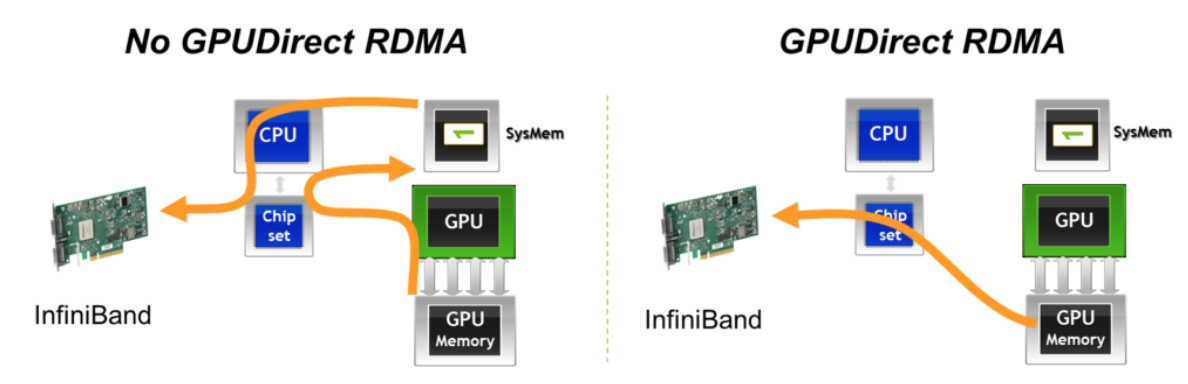
\includegraphics[width=0.49\textwidth]{gpu-rdma.png}
\mycaption{GPUDirect RDMA}{The figure shows the data transfers with and without GPUDirect RDMA. 
}
\label{fig-rdma}
%\vspace{-20pt}
\end{figure}

\begin{figure}
\centering
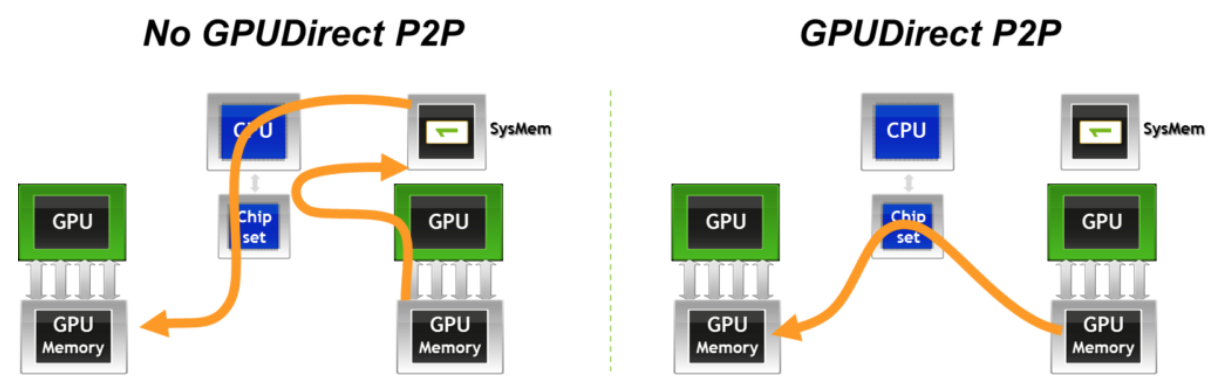
\includegraphics[width=0.49\textwidth]{gpu-ptp.png}
\mycaption{GPUDirect Peer-to-Peer}{The figure shows the data transfers with and without GPUDirect Peer-to-Peer. 
}
\label{fig-ptp}
%\vspace{-20pt}
\end{figure}


NVIDIA GPUDirect technologies provide high-bandwidth, low-latency communications with NVIDIA GPUs. GPUDirect is an umbrella name used to refer to several specific technologies. In the context of MPI the GPUDirect technologies cover all kinds of inter-rank communication: intra-node, inter-node, and RDMA inter-node communication. The newest GPUDirect feature is support for Remote Direct Memory Access (RDMA), with which buffers can be directly sent from the GPU memory to a network adapter without staging through host memory. This is shown in Figure~\ref{fig-rdma}. Another variant is GPUDirect for Peer-to-Peer (P2P) transfers, which can accelerate intra-node communication. Buffers can be directly copied between the memories of two GPUs in the same system with GPUDirect P2P. This is shown in Figure~\ref{fig-ptp}. 

If GPUDirect RDMA or GPUDirect P2P is available, the buffers can be directly transferred from the source to the destination without touching the host memory at all. This saves a lot of overhead in serializing/deserializing data and also copying of data between CPU and GPU buffers. Furthermore, the GPUDirect technology can be used along with Unified Virtual Addresses, which further eases the implementation as we do not have to worry about the location of the buffers that are being transferred. 

\subsection{GPUDirect in Gluon}
We attempted to implement the GPUDirect P2P and GPUDirect RDMA transfers in the Gluon Substrate, for transferring the data between GPUs of a single node in the context of the bfs\_push application. As explained before, when a source node tries to transfer data to a destination node, the following steps occur:
\begin{enumerate}
\item The offset data of the graph and the bitset data of the graph are computed at the GPU of the source
\item The offset data, bitset data and the shared graph data are copied and serialized into a CPU buffer at the source
\item The CPU buffer is transferred from the source to the destination
\item The CPU buffer at the destination is deserialized and copied to the GPU at the destination
\item The corresponding graph data, offset data and bitset data is computed at the GPU of the destination
\end{enumerate}
Using the GPUDirect Technology in this workflow, we can greatly reduce the overheads in these transfers, to the following steps:
\begin{enumerate}
\item The offset data of the graph and the bitset data of the graph are transferred using MPI at the source
\item The shared graph data is transferred using MPI at the source
\item The offset and bitset data is received through MPI at the destination
\item The shared graph data is transferred using MPI at the destination
\end{enumerate}
Note that all the steps can occur simultaneously along with other computations at the CPU of source and destination. The data transfers occur asynchronously without any CPU involvement. This feature, if applied effectively, has the potential to significantly improve the performance of data transfers, as compared to the other two features.

\subsection{Discussion and Limitations}
[TODO Hochan]